%% LyX 2.1.4 created this file.  For more info, see http://www.lyx.org/.
%% Do not edit unless you really know what you are doing.
\documentclass[unicode,pdfcover]{scutthesis}
\usepackage{fontspec}
\usepackage{color}
\usepackage{array}
\usepackage{longtable}
\usepackage{graphicx}
\usepackage[unicode=true,
 bookmarks=true,bookmarksnumbered=true,bookmarksopen=false,
 breaklinks=false,pdfborder={0 0 1},backref=false,colorlinks=true]
 {hyperref}
\hypersetup{pdftitle={博士论文标题},
 pdfauthor={你的名字},
 pdfsubject={华南理工大学博士学位论文},
 pdfkeywords={关键字1, 关键字2},
 unicode=false,linkcolor=blue, anchorcolor=black, citecolor=olive, filecolor=magenta, menucolor=red, urlcolor=magenta, pdfstartview=FitH}

\makeatletter

%%%%%%%%%%%%%%%%%%%%%%%%%%%%%% LyX specific LaTeX commands.
\providecommand{\LyX}{\texorpdfstring%
  {L\kern-.1667em\lower.25em\hbox{Y}\kern-.125emX\@}
  {LyX}}
%% Because html converters don't know tabularnewline
\providecommand{\tabularnewline}{\\}

\makeatother

\usepackage{listings}
\usepackage{xunicode}
\renewcommand{\lstlistingname}{列表}

\begin{document}

\title{Latex 与 Lyx 排版研究}


\author{徐川页}


\supervisor{指导教师:高德纳\ 教授}


\institute{华南理工大学}


\date{2010年4月13日}

\maketitle
\frontmatter
\begin{abstractCN}
论文排版对科技工作者来说一直是一个公认的繁琐事情。使用\LaTeX{}排版的突出缺点是控制符和文本符同时显现,容易干扰用户文本内容输入。鉴于此,本文提出了一种新颖的\LyX{}+Xe\LaTeX{}+\LaTeX{}组合的论文排版编辑方式。该排版方式取\LyX{}之长弥补\LaTeX{}的不足点,使得同时具有MS\ Word和\TeX{}排版两方面优势,同时基于Uincode的Xe\LaTeX{}引擎不仅使得文字兼容性增强,而且使用更方便。本文还以设计一套符合华南理工大学博士论文规范的\LaTeX{}/\LyX{}模板为例,验证了该组合方式的可行性。
\end{abstractCN}

\keywordsCN{\LaTeX{};\LyX{};排版;论文}
\begin{abstractEN}
Typesetting is a long-standing notorious troublesome for the scientific
researchers. The noticeable drawback in \LaTeX{} typesetting is that
control characters and text characters appear in the same time, likely
breaking user to input text. In view of this, we propose a novel combination
of \LyX{} + Xe\LaTeX{} + \LaTeX{} in editing paper. In this way, \LaTeX{}
learnes from Lyx's strong points to offset its weakness, with advantages
of both MS Word and \TeX{} typesetting. In additional Xe\LaTeX{} engine,
based on Uincode, not only improves compatibility but also makes it
more convenient to be used. This work also presents a set of \LaTeX{}/\LyX{}
templates of South China University of Technology doctoral thesis,
in order to verify the feasibility of the combination.
\end{abstractEN}

\keywordsEN{\LaTeX{}; \LyX{}; Typesetting; Paper}

\tableofcontents{}

\listoftables


\listoffigures



\chapterx{主要符号对照表}

【本节论文规范为可选,如果你的论文没有相关内容那么去除这一节;如果有,则删除这一行注释。】

\begin{table}
\centering{}%
\begin{tabular}{l>{\centering}p{2.5cm}l}
$Q$ - 系统最大取向数  &  & $d_{MC}$ - 网格常数(m)\tabularnewline
$\varepsilon_{e}$ - 弹性应变 &  & $k$ - Blozmann常数$\left(J/K\right)$\tabularnewline
 &  & \tabularnewline
 &  & \tabularnewline
 &  & \tabularnewline
\end{tabular}
\end{table}



\chapterx{英文缩略词}

【本节论文规范为可选,如果你的论文没有相关内容那么去除这一节;如果有,则删除这一行注释。】

\begin{table}
\centering{}%
\begin{tabular}{ccc}
SCUT  & South China University of Technology & 华南理工大学\tabularnewline
 &  & \tabularnewline
 &  & \tabularnewline
 &  & \tabularnewline
 &  & \tabularnewline
\end{tabular}
\end{table}


\mainmatter


\chapter{绪论}


\section{研究意义}

\TeX{}/\LaTeX{}是一种专业的科技文献排版语言,使用它写文档具有如下优势:
\begin{enumerate}
\item 将文档内容书写与格式排版的工作分离,使得专注与内容书写成为可能;
\item 基于编程化控制修改排版格式,工作灵活性和精确度高;
\item 基于独立操作系统的文档格式,兼容性好。
\end{enumerate}
但还存在一些不足之处,也就是\TeX{}\cite{knuth1986thetexbook}文档书写没有做到排版控制和内容完全分离。在编辑文档时,用户无法避免\TeX{}/\LaTeX{}\cite{goossens1994thelatex}格式控制符号和内容字符同时显示在眼前,因此这样会使得控制符号非常容易干扰用户输入文章内容,影响文章主题思路的书写。还有\TeX{}控制符种类繁杂,而且至今出现了大量衍生宏(典型的如\LaTeX{}),在方便用户编辑的同时,也大大增加了用户记忆负担。

最近兴起的\LyX{}排版软件系统可使得用户不再需要直面大量\TeX{}/\LaTeX{}控制符也可以得到\TeX{}/\LaTeX{}排版过的文档。它自动调用\TeX{}/\LaTeX{}引擎最终生成常见的ps、html和pdf等各种常见格式。该系统兼顾\TeX{}与MS
Word排版两者的优势\cite{lamport1994latexa},内容独立编辑格式的程度非常高。

学位论文是典型的科技文献,其具有规范的科技文献排版要求,特别是理工类学位论文需要大量的公式和文档排版,工作量非常大。因此研究如何提高学位论文编辑排版工作的效率有非常重要的现实意义。本文结合\LyX{}与\LaTeX{}文档编辑的特点,将\LyX{}与\LaTeX{}用在学位论文编辑排版工作,研究如何使用这种方法确实提高论文编辑的效率,最大程度地解决论文排版这类事情的繁琐性。


\section{本文的贡献}

本文立足于\LyX{}与\LaTeX{}可互为补充的这个特性,把握Xe\LaTeX{}引擎在字体处理方法的优势,提出了一种新颖的\LyX{}+Xe\LaTeX{}+\LaTeX{}组合的论文编辑方式。该排版方式取\LyX{}之长弥补\TeX{}/\LaTeX{}的不足点,使得同时具有word和\TeX{}排版两方面优势,而且基于Uincode的Xe\LaTeX{}引擎不仅使得文字兼容性增强,使用复杂度也大大降低。

为了验证该方式的可行性,本文以华南理工大学博士学位论文为例,为其设计了一套规范的\LaTeX{}宏和\LyX{}模板,采用Xe\LaTeX{}引擎可一键生成最终pdf文件,用户不再强制关注底层\LaTeX{}控制符,在\LyX{}中\LaTeX{}公式之类的编辑非常方便,所有学位论文排版格式化工作由本文设计的宏和模板来完成,使用户的集中力在于论文的内容上。

另一方面,由于缺乏系统性的优秀教程,特别是中文文档,要熟练掌握\LaTeX{}/\LyX{}书写文档却不是一件很容易的事情,本文将对这方面的问题进行详细阐述,突出思想性和指导性,降低入门槛,使得迅速掌握\LaTeX{}/\LyX{}编辑文档成为可能。


\chapter{\protect\LaTeX{}与Lyx排版简介}


\section{\protect\TeX{}/\protect\LaTeX{}概要}

\TeX{}排版语言由D. Knuth发明,1978年首次发布以来,得到了广泛的应用\cite{TUG},由于需求的多样性,在引擎、宏包、字体库和发布版方面出现了各种分支发展,这里简要列举如下:
\begin{enumerate}
\item 语言:\TeX{}的排版标识(指令)。
\item 引擎:\TeX{}(最早的\TeX{}解释器)、\LaTeX{}、PDF\TeX{}/PdfLatex、Xe\TeX{}/Xe\LaTeX{}、Lua\TeX{}等;
\item 宏包:plain \TeX{}、AMS-\TeX{}、\LaTeX{}、LAMS-\TeX{}、Con\TeX{}t等;
\item 中文字库:CJK、CCT、XeCJK;
\item 发行版:tetex、texlive、Mitex、CTex。
\end{enumerate}
Tex是可扩展的排版语言,通过宏包可以增强指令功能和多样化排版格式。\LaTeX{}就是一个最流行\TeX{}宏库,为了方便起见,本文中常用\LaTeX{}代替\TeX{}名词使用。注意有些宏包突破了基本\TeX{}规范,因此需要特别的引擎来处理。引擎就像编译器,最基本的\TeX{}引擎只可以生成dvi文件,但通过增强型\TeX{}引擎,如PDF\TeX{}和Xe\TeX{}都能编译\TeX{}文件直接生成pdf文件。Xe\TeX{}和Xe\LaTeX{}都是基于Unicode字体的\TeX{}增强型引擎,不同的是一个编译\TeX{}源码,另一个编译\LaTeX{}源码。整个\TeX{}工作体系架构见图\ref{fig:tex_work_framework}。

\begin{figure}
\centering{}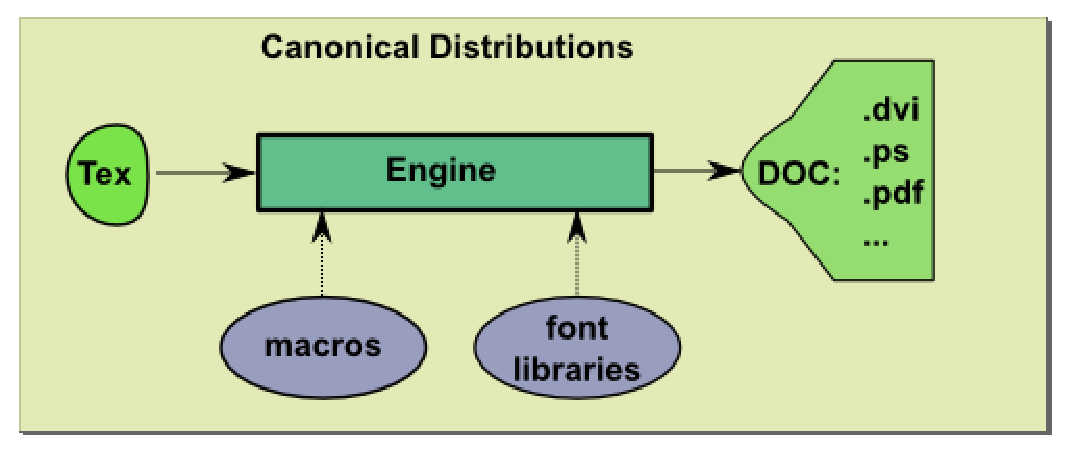
\includegraphics[scale=0.7]{figure/tex_engine}\caption[如果图题太长,在这里写个短标题只在图索引中出现]{\label{fig:tex_work_framework}\protect\TeX{}工作体系框架}
\end{figure}


用\LaTeX{}可以输入复杂的排版公式,如\eqref{eq:cx1}式。
\begin{equation}
\frac{\partial\,P(S_{j},\,t)}{\partial t}=\sum_{i}P(S_{i},\,t)W(S_{i}\rightarrow S_{j})-\sum_{i}P(S_{j},\,t)W(S_{j}\rightarrow S_{i})\label{eq:cx1}
\end{equation}


也可以输入表格如表 \ref{tab:example}。

\begin{table}
\caption{\label{tab:example}实例表}


\centering{}%
\begin{tabular}{c|c|c|c|c}
\hline 
case & Method1 & Method2 & Method3 & 产出\tabularnewline
\hline 
1 & 32 & 34 & 23 & 34\tabularnewline
\hline 
2 & 12 & 324 & 23 & 234\tabularnewline
\hline 
3 & 23 & 34 & 34 & 23\tabularnewline
\hline 
4 & 12 & 23 & 34 & 23\tabularnewline
\hline 
\end{tabular}
\end{table}



\subsection{关于\protect\LaTeX{}宏包的设计}

设计宏的源文件一般含.ins和.dtx两个文件,再调用\LaTeX{}工具命令生成.cls和.sty文件,当然我们可以直接设计.cls和.sty,无非.ins和.dtx多了一些安装说明和文档说明。

刚开始学\TeX{}和LATEX推荐阅读参考文献\cite{lshort,lamport1994latexa}。


\section{Lyx工具简介}

\LyX{}是一种半所见所得文档编辑工具,能够支持\TeX{}文档编辑。在\LyX{}主窗口输入用户文字内容,通过菜单命令将文档转换为\TeX{}格式,再在后台调用\LaTeX{}或其他引擎如Xe\LaTeX{}来编译成为最终文档。

\LyX{}的体系包含三大组成部分:
\begin{enumerate}
\item \TeX{}/\LaTeX{} 宏:\LyX{}会收集系统上已经存在的\TeX{}/\LaTeX{}宏,这些宏在\LyX{}的layout文件中调用。
\item 文档class\ and\ Layout:Layout主要规定\LyX{}用户输入界面文档显示的格式,这些格式没有必要和\LaTeX{}的生成格式但推荐一致。Linux系统下,在\textasciitilde{}/.lyx/layouts目录下可以定义自己的layout文件,可以通过菜单栏Document->settings->document\ class来选择。当前最新版可以在Document->settings->document\ class中使用“local\ layout”选择使用本地目录下的lyx\ layout文件,如“scutthesis.layout”。\LyX{}菜单上的help->customization\ layout的作用有两个:调用用户指定的tex\ class和设置\LyX{}文本界面段落格式。 
\item Template:其实就是一个正常的\LyX{}文件,作为一个模板,保存了一些相应的基本设置,这样你下次在需要此类格式的文档时,只要在该模板的基础上次新建即可。
\end{enumerate}
另外,如果你的要求不太高,完全可以把\LyX{}当成一个\LaTeX{}的草稿本,因为\LyX{}可以方便导出\LaTeX{}格式文档。


\section{Xe\protect\LaTeX{}引擎简介}

字体设置一直是\TeX{}排版处理的核心内容也是最难的方面。不仅用户使用起来麻烦,各\TeX{}引擎处理起来也常出现字体不兼容的问题。因此解决字体处理问题显得很重要。Xe\TeX{}使用Unicode字符编码方式以试图解决字体处理上出现的问题。它可以脱离Tex内核字体来使用,支持OpenType和系统自带字体,支持和使用新字体非常方便。Xe\TeX{}已经捆绑在\TeX{}\ Live\ 2010、Mac\TeX{}\ 2010和MiK\TeX{}\ 2.8等发行版中。就像Xe\TeX{}是\TeX{}的增强一样,Xe\LaTeX{}是\LaTeX{}的增强。既然是对\LaTeX{}语言规范的增强,就有相应的扩展引擎,即Xe\LaTeX{}引擎。常见使用Xe\LaTeX{}来处理文档。


\subsection{关于字体的设置}

\LaTeX{}中的字体有五种属性,\LaTeX{}含有相关命令可以来分别设置\cite{latex2efontsel}。同样Xe\LaTeX{}也可以分别设置英文字体和中文(CJK)字体。

对于英文字体的常见设置如下:

\textbackslash{}setmainfont\{\TeX{} Gyre Pagella\} \%英文缺省字体,用 \textbackslash{}rmfamily
所对应到的字体

\textbackslash{}setmonofont\{Monaco\} \%英文等宽字体, \textbackslash{}ttfamily
所对应到的字体

\textbackslash{}setsansfont\{Trebuchet MS\} \%英文无衬线字体,\textbackslash{}sffamily
所对应到的字体

\textbackslash{}newfontfamily:这个命令可以自行定义类似 \textbackslash{}rmfamily
之类的字型选择命令。 

对中文(这里CJK包括中文)常见设置如下:

\textbackslash{}setCJKmainfont{[}BoldFont=\{SimHei\}{]}\{SimSun\}\%中文缺省字体 

\textbackslash{}setCJKmainfont{[}BoldFont=\{Adobe Heiti Std\},ItalicFont=\{Adobe
Kaiti Std\}{]}\{Adobe Song Std\} 

\textbackslash{}setCJKmonofont\{Adobe Fangsong Std\}

\textbackslash{}setCJKmonofont\{YouYuan\}\% 设置代码或数学公式出现的中文字体

\textbackslash{}setCJKfamilyfont\{song\}\{AR PL SungtiL GB\}\%重命名一种新字体song,调用方式:\textbackslash{}CJKfamily\{song\}
这是些文本。

xeCJK 是一个Xe\LaTeX{} 宏包,用于排版CJK 文字,包括字体选择和标点控 制等。调用方式:

\textbackslash{}usepackage{[}Options{]} \{xeCJK\} 

可用的Options:

BoldFont: 启用CJK 粗体字

SlantFont: 启用斜体字slshape 

CJKnumber: 调用CJKnumb 

宏包 CJKchecksingle: 避免单个汉字单独占一行。

Xe\TeX{}控制命令:

\textbackslash{}Xe\TeX{}linebreaklocale\ “zh”是表示Xe\TeX{} 应该以中文的方式断行,因为一般英文字只会在空白处断行,而中文字除了避头避尾以外可以断在任何地方,因此要指定Xe\TeX{}
使用中文方式断行。

\textbackslash{}Xe\TeX{}linebreakskip 则是让Xe\TeX{} 可以在字元间加入0pt\textasciitilde{}1pt
的弹性间距,这样才能排出左右切齐的文件。

Xe\TeX{} 本身就提供选择字型的指令,不过还是提供了fontspec package 来简化过程,以下是一些重要的基本指令:

为了和CJKnumb, CJKulem,CJKfntef等兼容xeCJK重新定义了CJK 部分宏命令,如\textbackslash{}CJKfamily,
\textbackslash{}CJKsymbol, \textbackslash{}CJKpunctsymbol 注意xeCJK不需要CJK支持并且xeCJK会自动禁止加载CJK宏包。


\subsection{Texmaker中调用Xe\protect\LaTeX{}}

Texmaker是一个自由跨平台Latex编辑器\cite{Texmaker},常见于Linux系统下。它支持unicode字符编码,内置pdf预览。

我们可以设置Texmaker调用Xe\LaTeX{}引擎代替普通的\LaTeX{}引擎,编译扩展后的\TeX{}文档。设置方法:

打开文件 \%appdata\%\textbackslash{}xm1\textbackslash{}texmaker.ini\textquotedbl{}
修改如下:

\begin{lstlisting}
User\ToolName1=XeLaTeX
User\Tool1="xelatex -interaction=nonstopmode %.tex"
\end{lstlisting}



\subsection{Lyx中调用Xe\protect\LaTeX{}\label{sub:LyX_XeLaTeX}}

Lyx2.0以后的版本默认支持Xe\LaTeX{}编译,而早期\LyX{}版本如1.6.7必须自行在toolbar上加入一些功能调用按钮,如view\ PDF(xelatex)等菜单命令。如何在\LyX{}下调用xetex编译\LaTeX{}文档,参加\LyX{}官方wiki\cite{xetex_lyx}。


\chapter{博士论文模板设计}


\section{Lyx+Xe\protect\LaTeX{}+\protect\LaTeX{}组合方式}

\LaTeX{}是一个所见非所得的方式,使用起来不是那么直接,入门槛很高,而\LyX{}是半所见所得的编辑工具,可将用户的文档内容变化为Tex文档,再在后台调用\TeX{}引擎生成最终文档。这样不需要使用很多\LaTeX{}的控制符。而Xe\LaTeX{}作用为一种扩展的\TeX{}引擎,它可以使用系统自带的字体,如中文用户不需要自己去配置CJK包,免去了很多麻烦。支持unicode字符统一处理,这是处理非英文\TeX{}文档最彻底的解决方式。考虑到以上优势,我们将利用这种方式处理华南理工大学博士学位论文排版编辑。


\section{华南理工大学博士论文排版设计}

华南理工大学博士论文书写规范包括版面、段落、字体、页眉页脚、参考引用等方面的要求,详见华南理工大学《硕/博士研究生论文答辩及学位申请工作手册》。

本文模板设计(scutthesis)的主要思想为\emph{简洁而易于维护}。具体如下:
\begin{enumerate}
\item 论文封面是通过maketile生成,有内置简单版和外部pdf导入版两种,在调用scutthesis.cls时加入pdfcover选项将使用pdf导入封面,它会将本地目录下名为thesis\_cover.pdf的文件作为封面页,该pdf文件一般包含中英文封面及原创说明等\emph{摘要前的内容},这些pdf页会被合并到\LaTeX{}源码中一起编译,直接包含外部pdf作为封面避免了一些繁琐的细节问题,减轻用户的使用困难。该thesis\_cover.pdf可以从填好的微软.doc文件转换而来\footnote{Linux下用openoffice,window下用MC word将.doc转为.pdf文件},word页面可以到“研究生院主页网站->学位办公室->下载区”下载最新“研究生学位论文撰写规范”文档中找到。使用这种方式注意力将集中到论文的正文部分,这点不同于现存的各高校\LaTeX{}模板。如果在调用scutthesis模板类之前没有使用pdfcover选项,将使用内置简单封面(适用于草稿模式)。
\item 由于博士论文是中英文混合排版,也不排除用其他语言文字(如留学生的使用),因此要支持各种语言字体是一种要求,这样最优的选择是采用Unicode来编码,而不仅是CJK。据于此,本模板设计将采用基于Unicode和Opentype字体的Xe\LaTeX{}来完成设计。xeCJK是宏包,Xe\TeX{}是引擎,两者虽然都支持中文编辑,但XeTex是内核上实现,比一些辅助的中文包之类的东西(CCT或CJK之类)更可靠,因此Xe\TeX{}将更有发展潜力。使用\LyX{}+Xetex最大好处是支持各种语言排版,只需一点额外的切换配置可以支持中文。还有,不采用CTex宏来设计框架的原因是避免用户和维护人员去学习复杂的CTex的定义,较早的CASThesis.cls就是基于CTex设计而来,总体感觉繁琐难读,不宜维护。
\end{enumerate}

\section{LaTex模板设计}

首先设计一个符合华南理工大学学位论文规范的\LaTeX{}库,包括cls文件(scutthesis.cls)和参考文献样式文件bst(scutthesis.bst,符合国标GBT7714风格),其中cls文件还必须支持中文Tex排版。\TeX{}中处理中文牵涉到三个必须要解决的问题

1. 提供可用的中文字库,如宋体(simsum),关于Ubuntu下安装中文字体见附录 \ref{sec:ubuntuzhfont}。

2. \TeX{}宏和编译器支持中文文本的处理,关于Texlive发行版的安装见附录 \ref{sec:texlive_install}。

3. \TeX{}编辑器支持中文文本的处理

处理中文有几套常规思路:
\begin{itemize}
\item 利用CJK+pdfLatex/Xe\LaTeX{}
\item 利用xeCJK+Ctex+Xe\LaTeX{}
\end{itemize}
本模板设计做到兼顾性能和方便性,设计思路采用xeCJK+Xe\LaTeX{}组合方式。这样尽量避免去纠缠CTex宏包,当然不排除使用它的设计思想。

模板的外观表现和功能都放在scutthesis.cls中,在对外观进行细微调整时,只需要更新这两个文件,不需要对.tex源文件做修改。这也给模板更新带来了极大方便。
\begin{itemize}
\item 该模板的功能要点: 
\item 使用XeTEX 引擎处理中文; 
\item 包含中文字符的源文件(.tex, .bib, .cfg),编码都使用UTF-8;
\item 使用Bib\TeX{} 管理参考文献。参考文献表现形式(格式) 受.bst 控制,方便在不同风 格间切换,目前生成的列表符合国标GBT7714
要求;
\item 可以直接插入EPS/PDF/JPG/PNG 格式的图像,并且不需要bounding box 文件(.bb);
\item 模板的格式受scutthesis.cls 控制,方便模板更新和模板修改。
\end{itemize}
scutthesis的\LaTeX{}宏包部分参考过的模板:

1. 清华大学学位论文\LaTeX{}模拟http://thuthesis.sourceforge.net/

2. 同济大学:http://tongjithesis.sourceforge.net/

3. 东南大学学位论文\LaTeX{}模板http://code.google.com/p/seuthesis/

4. 上海交大http://bbs.sjtu.edu.cn/bbstdoc?board=tex\_latex


\section{Lyx模板设计}

有了\LaTeX{}的cls/bst文档(这里为scutthesis.cls和scutthesis.bst),就可以用\LaTeX{}来设计博士论文了,如Ubuntu下用Texmarker作为\LaTeX{}的编辑器,它可以调用Xe\LaTeX{}引擎生成pdf。但这样设计而来的\LaTeX{}文档是一个用户非友好的,直观结构层次不明显。进一步,因此我们借助\LyX{}来弥补这个缺陷。由于\LyX{}需要用到cls文档,所以\LyX{}模板设计要在博士论文的\LaTeX{}宏cls文件设计好后才方便。

\LyX{}的相关博士论文模板,主要有两个:\LyX{} layout(scutthesis.layout)和内容输入模板(scutthesis.lyx)。


\section{总体设计框架}

本设计包括两部分:\LaTeX{}模板类和\LyX{}模板布局。其流程框架、模板使用和文件关系如图\ref{fig:scutthesis_framework}。

\LaTeX{}模板类包括文本排版类scutthesis.cls和参考文献样式scutthesis.bst。在传统的\TeX{}使用方式中(way\ 1),先用\TeX{}编辑器直接输入你的论文内容(参照例子scutthesis.tex格式),再运行Xe\LaTeX{},其调用scutthesis.cls和scutthesis.bst就可以格式化为符合华南理工大学学位论文的排版要求。注意摘要之前的几页排版内容,如标题和版权页,是以pdf文件方式包括在tex文件中,发布包中提供了相应的word
.doc版文件,请自行修改再转换为pdf文件。 

你也可以通过\LyX{}间接地使用\LaTeX{}模板类(way\ 2),不需要直面\LaTeX{}源代码。在\LyX{}中采用scutthesis.layout布局,输入你的论文内容如scutthesis.lyx格式,再一键调用Xe\LaTeX{}自动编译成scutthesis.tex文件,并加入scutthesis.cls和scutthesis.bst生成最终的pdf文件。
详细的设计内容,见发布包中的scutthesis.pdf文件。

\begin{figure}
\begin{centering}
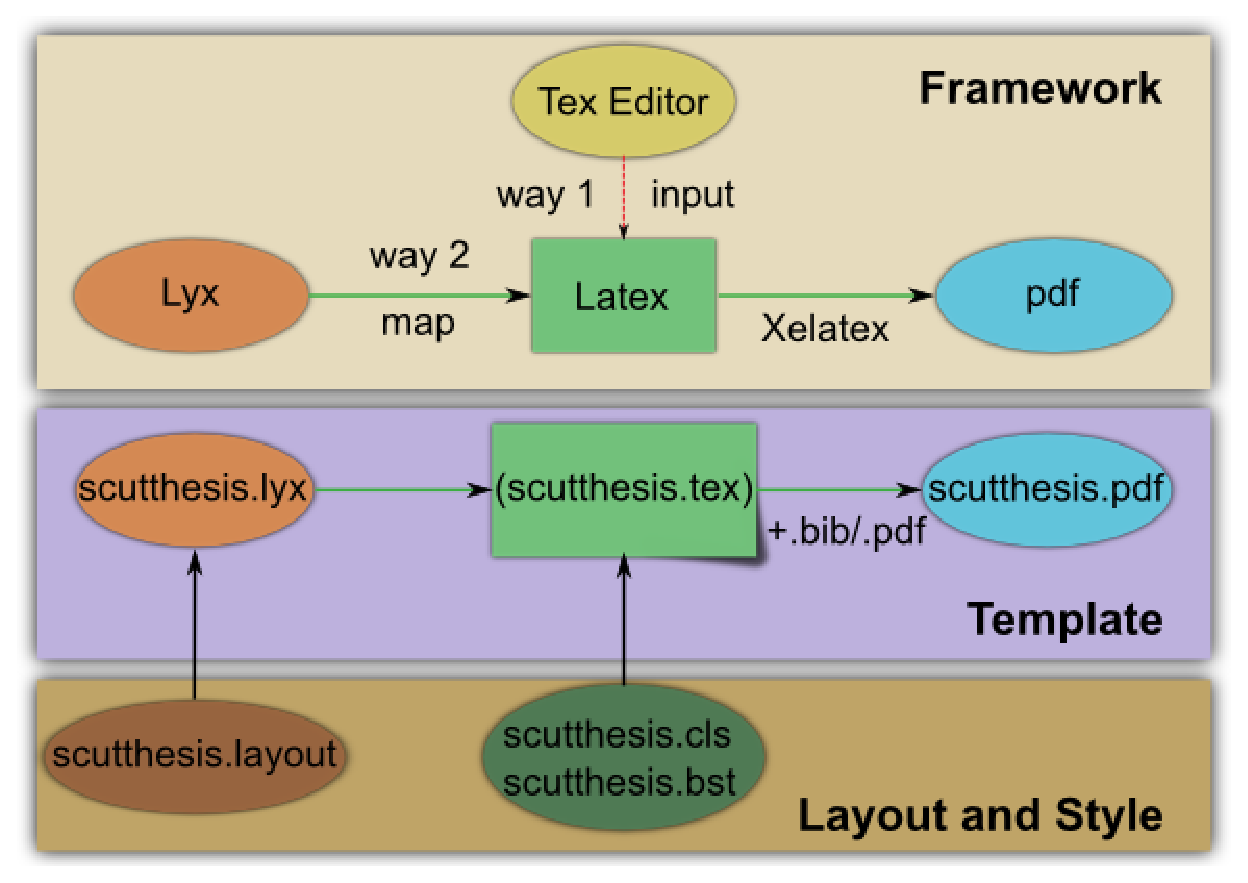
\includegraphics[scale=0.6]{figure/scutthesis}
\par\end{centering}

\caption{\label{fig:scutthesis_framework}流程框架、模板使用和文件关系}
\end{figure}


本设计的源码下载地址为:https://github.com/alwintsui/scutthesis 。


\chapter{博士论文模板的使用}


\section{使用之前}

由于Latex和Lyx模板与操作系统平台无关,它们可以在Windows、Ubuntu和Mac\ OS\ X等系统下使用。scutthesis是基于XeTex(Xe\LaTeX{})开发的,无论是\LyX{}还是Latex都需要scutthesis的LATEX模板正确安装,为了方便使用,我们在本地目录调用scutthesis.cls、scutthesis.bst和scutthesis.layout。当也可以将cls和bst安装在Latex/TEX的系统默认路径下,如Ubuntu系统下的\textasciitilde{}/texmf或/usr/local/share/texmf目录。


\section{Latex模板使用}

如果是直接使用latex命令,建议新建批处理文件,内容如下

Linux和Mac OSX系统下

\begin{lstlisting}
#!/bin/sh
rm scutthesis.pdf *.aux *.lo? *.toc *.ind *.inx *.gls *.glo *.ist *.idx *.ilg *.out *.bak *.bbl *.brf *.blg *.dvi *.xdv *.ps body/*.aux
xelatex -no-pdf --interaction=nonstopmode scutthesis 
bibtex scutthesis 
bibtex scutthesis 
xelatex -no-pdf --interaction=nonstopmode scutthesis 
xelatex --interaction=nonstopmode scutthesis 
evince scutthesis.pdf 
\end{lstlisting}


Windows系统下

\begin{lstlisting}
del *.aux *.lo? *.toc *.ind *.inx *.gls *.glo *.ist *.idx *.ilg *.out *.bak *.bbl *.brf *.blg *.dvi *.ps *.xdv body\*.aux
del scutthesis.pdf 
xelatex -no-pdf --interaction=nonstopmode scutthesis
bibtex scutthesis 
bibtex scutthesis 
xelatex -no-pdf --interaction=nonstopmode scutthesis 
xelatex --interaction=nonstopmode scutthesis 
\end{lstlisting}


其他系统仿照使用。


\subsection{模版使用框架 }

直接使用Latex编写论文,可以采用如下结构布局

\begin{lstlisting}
\documentclass[unicode,pdfcover]{scutthesis}
\usepackage[unicode=false,bookmarks=true,bookmarksnumbered=true,bookmarksopen=false,
 breaklinks=false,pdfborder={0 0 1},backref=false,colorlinks=true]
 {hyperref}

\hypersetup{
 pdftitle={SCUT Thesis title},
 pdfauthor = {your name}
 pdfkeywords={keyword1, keyword2},  
 pdfstartview=FitH,
 unicode=false,
 linkcolor=blue,anchorcolor=black,citecolor=olive,filecolor=magenta,menucolor=red,urlcolor=magenta,
}
\begin{document}

\maketitle % include thesis_cover.pdf covered from word doc
%%%%%%%%%%%%%%%%%%%%
\frontmatter %Roman numerals for page numbering
\include{body/abstract} % Chinese/English abstract
\tableofcontents{} 
\listoftables
\listoffigures
\include{body/symbols} 
\include{body/abbreviation} 
%%%%%%%%%%%%%%%%%%%
\mainmatter %Arabic numerals for page numbering
\include{body/chapter01} 
\include{body/chapter02}
\include{body/chapter03} 
\include{body/chapter04}
\backmatter %no chapter numbering but page number continues.
\include{body/conclusion}
\bibliographystyle{scutthesis} 
\bibliography{reference/scutthesis,reference/chap3}
\include{body/appendix} 
\include{body/pub} 
\include{body/ack}
\end{document}
\end{lstlisting}
scutthesis需要使用unicode 编码,

\begin{lstlisting}
\documentclass[unicode]{scutthesis}
\end{lstlisting}


硕/博论文选择:默认是博士论文,使用以下命令定义硕士论文类型,

\begin{lstlisting}
\documentclass[unicode,master]{scutthesis} 
\end{lstlisting}


pdfcover选项将在maketitle中调用thesis\_cover.pdf,如果没有pdfcover将需要在\textbackslash{}begin\{document\}之后设置调用\textbackslash{}title、\textbackslash{}author、\textbackslash{}supervisor、\textbackslash{}institute和\textbackslash{}date指令设置基本信息,例如:

\begin{lstlisting}
\title{Latex 与 Lyx 排版研究}
\author{徐顺}
\supervisor{指导教师:高德纳 教授}
\institute{华南理工大学}
\date{2010年4月13日}
\end{lstlisting}


使用内置简单封面可加快latex 的编译速度,适合草稿模式。

\begin{lstlisting}
\documentclass[unicode,pdfcover]{scutthesis} 
\end{lstlisting}


还可以设置pdf 文件属性,打上你自己的烙印

\begin{lstlisting}
\hypersetup{ 
unicode=true,
pdftitle={论文的题目}. % 题目 
pdfauthor = {你的名字},% 作者
}
\end{lstlisting}


如果pdf目录书签中的中文乱码,将unicode选项设置false试试。


\subsection{新建章节}

全文的章节顺序为:封面页-中文摘要-英文摘要-表格目录-插图目录-主要符合对照表-英文缩略词-正文第一章绪论-正文第二章-...-正文结论-参考文献-附录-发布论文列表-致谢。

中文摘要到正文绪论之前是使用罗马数字页码,正文以下都是使用阿拉伯数字页码。

图表目录清单、主要符号表和英文缩略词在必要时使用。\emph{主要符合对照表}和\emph{英文缩略词}章节是通过\textbackslash{}preface命令控制,即

\textbackslash{}preface\{主要符号对照表\}和\textbackslash{}preface\{英文缩略词\}。 

正文的章节使用\textbackslash{}chapter,例如:\textbackslash{}chapter\{绪论\} 

新建一章的第一级小节命令:\textbackslash{}section\{新建章节\}。

多级章小节用\textbackslash{}subsection\{3.2.1\},\textbackslash{}subsubsection\{3.2.1.1\}。

不建议使用超过4级的小节。若有需要可以使用没有编号的章节题目。使用‘{*}’ 去掉编号,命令\textbackslash{}subsubsection{*}\{无编号章
节\},

附录为可选章节,新建附录格式为

\textbackslash{}appendix\{附\textbackslash{}quad 录\}\%

\textbackslash{}section\{随机数的生成\}\%第一个附录章节

添加多个附录章节,使用\textbackslash{}section和\textbackslash{}subsection等等。

一般是自动首行空两格,但碰到列表项后的段落,不会首行自动空两格,latex文档中可用\textbackslash{}qquad\{\},而在lyx文档中使用菜单插入:insert->foramtting->Horizontal
space选择double Quad(2em)。


\subsection{插入图片}

Latex一般插图格式为

\begin{lstlisting}[language=TeX]
\begin{figure}[H] 
\centering
\includegraphics[scale=0.4]{figure/scutlogo.eps}
\FigureBicaption{华工}{SCUT} 
\label{fig:single} 
\end{figure}
\end{lstlisting}


其中{[}H{]} 参数强制固定浮动图形的位置; scale 参数可以调整图片大小; \textbackslash{}FigureBicaption\{中文标题\}\{英文标题\}
加入图片标题;\textbackslash{}label 命令用来引用图片。

插入子图也可参考

http://blog.sina.com.cn/s/blog\_5e16f1770100n206.html


\subsection{插入表格}

基本表格

\begin{figure}
\caption[这个标题会出现在索引中]{如果表格的标题很长,那么在表格索引中就会很不美观,所以要像chapter那样在前面用中括号写一个简短的标题。}


\centering{}%
\begin{tabular}{cc}
\hline 
文件名 & 描述\tabularnewline
\hline 
scutthesis.cls & 模板类文件\tabularnewline
scutthesis.bst & 参考文献Bibtex 样式文件\tabularnewline
\hline 
\end{tabular}
\end{figure}


模版还提供了更加复杂的表格功能,如表格中的斜线,注释等。本文档暂时不提供这 些复杂表格的例子,暂留给读者探索。


\subsection{公式与定理}

简单公式环境:

\[
y=mx+c
\]
公式太长,多行排列:

\begin{equation}
\label{eq:split} 
\begin{split}    
  y&=mx+c\\        & \quad(n+o)x+c\\        &=1  
\end{split} 
\end{equation}

多个公式并列不要用多个equation环境,会造成公式间距过大的问题,用gather环境:

\begin{gather} 
y=mx+c \label{eq:eq1}\\ 
x=(n-2)+d 
\label{eq:eq2} 
\end{gather}

模版提供了多种定理环境:命题(proposition),引理(lemma),定理(theorem),公理(axiom),推论(corollary),情形(case),猜想(conjecture),性质(property),还有定义(definition),例(example),注(remark)。下面以常见的环境作例子。
\begin{theorem}
中国人是人\end{theorem}
\begin{proof}
把证明内容放到\textbackslash{}begin\{proof\} 和\textbackslash{}end\{proof\} 
\end{proof}


\subsection{参考文献}

根据条目的类型,如@article,@procceedings,@book,BibTex会自动分别在文献题目后面加上{[}J{]},{[}C{]}和{[}M{]}等标识。也可以自己设定TypeofLit,给定文献类型,如引用网页的代码

\begin{lstlisting}
@MISC{google,
author = {Google}, 
title = {Home Page},
year = {},
TypeofLit = {EB/OL}, 
modifydate = {}, 
citedate = {},
url = {http :// www.google.com/},
language = {},
}
\end{lstlisting}
参考文献可以分章节管理,只需要在主文件中的参考文献中都包含进去就可 以,如\textbackslash{}bibliography\{chap1,chap2,...\}。

参考文献举例说明:关于书的\cite{Meta_CN,goossens1994thelatex},关于期刊的\cite{chen2007ewi,wang_model_2009},会议论文\cite{DPMG,cnproceed},硕士学位论文\cite{zhubajie},博士学位论文\cite{shaheshang},技术报告\cite{NPB2},电子文献\cite{xetex_lyx,Texmaker}。

如果参考文献中含有中乱码,可能是你的bib文件不是utf-8格式,需要用文档编辑器另存为utf-8格式,或者你也可以在bibtext的条目中增加一个域:language=\{zh\}。

关于文献参考引用,推荐使用专业的文献引用管理器,此类软件很多如endnote和zotero。


\subsection{交叉引用}

交叉引用需要两个步骤。 
\begin{enumerate}
\item 用\textbackslash{}label\{\} 命令标识;
\item 用\textbackslash{}ref\{\} 命令引用。
\end{enumerate}
从本节的例子可以看出,无论是图片,表格,公式,定理,算法,代码,章节等,都可以表示和引用。如\textbackslash{}label\{ch:intr\}和第\textbackslash{}ref\{ch:intr\}章。注意到,\textbackslash{}ref命令只是引用了编号,并没有给出引用的类型,因此需要加上引用类型的名字,再如算法
\textbackslash{}ref\{alg: life\}。公式的编号一般在括号里,特殊地,可以用\textbackslash{}eqref\{\}
代替‘(\textbackslash{}ref\{\})’。


\section{Lyx模板使用}

\LyX{}只是提供一种编辑框架,此模板提供scutthesis.layout让\LyX{}识别基于scutthesis类型的文档,真正文档的编译需要有Xelatex工具来完成。Ubuntu上的基本配置:
\begin{enumerate}
\item 把scutthesis项目发行包里面的 scutthesis.layout放置到主lyx文件的同目录或者路径 \textasciitilde{}/.lyx/layouts/scutthesis.layout;
\item 打开\LyX{}软件,新建主lyx文件(用于书写论文内容),点击运行:tools->reconfigure,之后在\LyX{}中的document->settings->document\ class下拉列表中能够找到book(SCUT\ Thesis)项,或者选择local\ layout打开文件选择scutthesis.layout,表示已经配置成功。
\item 如果是lyx2.0以下版本,其不支持基于文档的字体设置,那么需要注释掉\textasciitilde{}/.lyx/lyxrc.defaults文件中默认的西文T1编码:\#\textbackslash{}font\_encoding
\textquotedbl{}T1\textquotedbl{},注意每次reconfigure后\textasciitilde{}/.lyx/lyxrc.defaults内会还原。
\end{enumerate}
对于其他系统上的配置,可参照以上路径,做相应的路径修改即可完成。

调用Lyx模板写论文比直接用Latex简单直观多了,大部分格式可以参考scutthesis.lyx这个样本文件。

Document->settings...->PDF Properties中按照个人的情况修改Header Infomation的字段。

Aditional options的值通常情况下各链接的颜色可以不一致,如:

\begin{lstlisting}
unicode=false,linkcolor=blue, anchorcolor=black, citecolor=olive, filecolor=magenta, menucolor=red, urlcolor=magenta, pdfstartview=FitH
\end{lstlisting}


最后论文到图书馆提交时,要求链接颜色都设定为黑色,其值改如下另外生成一份文档:

\begin{lstlisting}
unicode=false,linkcolor=black, anchorcolor=black, citecolor=black, filecolor=black, menucolor=black, urlcolor=black, pdfstartview=FitH
\end{lstlisting}


注意在Windows系统下,pdf文件thesis\_cover.pdf的路径名用\textbackslash{}分隔符而不是/分隔符。

如果scutthesis.lyx导出的latex文件中,在scutthesis模板调用指令的选项中自动加入了english选项,如\textbackslash{}documentclass{[}english,unicode{]}\{scutthesis\},这会使得图表标题等使用英文的figure,table字符而不是“图”和“表”等对应的中文字符,多半是lyx文件中无意使用了英文环境。可以使用文本编辑器打开scutthesis.lyx文件,查找并删除“\textbackslash{}lang
english”语句即可。


\subsection{关于Lyx2.0的支持}

Lyx2.0做了一些有利于scutthesis(XeTex)格式的\href{http://wiki.lyx.org/LyX/NewInLyX20/}{功能升级}:
\begin{enumerate}
\item 开始支持Xe\TeX{}\ backend
\item 针对每个文档可个性化Output设置,支持PDF(XeTex)格式
\item 针对每个文档可个性化font encoding设置
\end{enumerate}
强烈推荐使用2.0以上版本,scutthesis完全可以不修改cls文件从Lyx1.6迁移到Lyx2.0,而且Lyx2.0中的配置使用几乎不需要特殊的配置。例如增加了\textbackslash{}default\_output\_format关键字,将菜单中view和update的命令改为和文档自动关联,我们可以把XeTex(也就是XeLaTex)作为scutthesis的一种默认输出格式。如果scutthesis的相关字体已经安装了,直接在lyx使用快捷键ctrl+R就可以生成论文pdf文件了。

Lyx2.0上的使用关键在于其设置,选择Document->settings...参考设置如下(\emph{以下设置都包含在scutthesis.lyx中,用户不需再次设置}):

Document class: book(SCUT Thesis) (对于scutthesis.lyx)

Class options/Predefined: unicode

Use noe-Tex fonts(via XeTex/LuaTex) \%选择这项,很重要

LaTex font encoding:None (no fontenc)

Paper Format/Format:Default

Page Margins/Default Margins: checked

Language:Chinese(simplified); 

Quote Style:\textquotedbl{}text\textquotedbl{} 

Encoding/other:Unicode(XeTex)(utf8)

Language package:None

Citation style:Default(numerical)

Use hyperref support:checked,

Header Information:修改为你自己的文档信息

Float Placement/Use default placement:checked 

LaTex Preamble:留空 

OutPut/Default Output Format:PDF(XeTex)

另外在File Handling中最重要的两种文件格式

File Formats: Latex(Xe\TeX{})后缀为 .tex和Pdf(XeTex)后缀为 .pdf

Converters: Latex(Xe\TeX{})->Pdf(XeTex): 设置为

xelatex \$\$i 

latex=xelatex 

在document设置是选择Default Output Format:PDF(XeTex)


\chapter{结论}

本文研究了一种新颖的\LyX{}+Xe\LaTeX{}+\LaTeX{}组合的科技文献排版方式,设计了第一个专业型华南理工大学\LaTeX{}/\LyX{}博士学位论文模板库,在全国高校学位论文模板中,首创支持Lyx论文编辑,实现了模板使用与操作系统平台无关,一键生成pdf文件的快捷方式。

总体来说,\LyX{}、Xe\LaTeX{}和\LaTeX{}组合实现了一种优势互补,使得科技文献的编辑排版工作量大为下降。

\bibliographystyle{scutthesis}
\bibliography{scutthesis}



\appendix{附录}


\section{Ubuntu Linux系统下中文字体的安装}

\label{sec:ubuntuzhfont}

整个过程分为两部分:得到中文字体文件和安装设置。

File `algorithm2e.sty' not found. 

sudo apt-get install texlive-science

常用中文字体有三套:

1. winfonts(微软的六种中易字体,包括宋体、黑体、楷书、仿宋、隶书、幼圆),

2. adobefonts(Adobe 的四套字体,包括 Adobe Song Std、Adobe Heiti Std、Adobe
Fangsong Std、Adobe Kaiti Std)

3. Ubuntu开源的文泉字体

CTex宏库默认支持winfonts和adboefonts。因此要在linux系统下使用Ctex宏库最好是安装这些字库之一。

将要按照的字体放置到默认搜索路径\textasciitilde{}/.fonts中,运行fc-cache -fv 命令更新字体缓存,然后执行
fc-list :lang=zh查看是否有新安安装字体。

网络上有介绍http://blog.chinaunix.net/u3/109488/showart\_2222797.html

从windows系统中拷贝如下字体到 \textasciitilde{}/.fonts/winfonts 目录中。

\begin{lstlisting}[language=bash]
:~/.fonts/winfonts$ls
arialbd.ttf ARIALNB.TTF ariblk.ttf cour.ttf SIMLI.TTF timesbi.ttf
arialbi.ttf ARIALNI.TTF courbd.ttf simfang.ttf simsun.ttc timesi.ttf 
ariali.ttf ARIALN.TTF courbi.ttf simhei.ttf SIMYOU.TTF times.ttf
ARIALNBI.TTF arial.ttf couri.ttf simkai.ttf timesbd.ttf 
\end{lstlisting}


这样以后你的系统就安装好ctex需要的winfonts。(除此之外,上面的字体中还包含了Times New Roman、Arial、Courier
New英文字体) 

\emph{注意:}scutthesis.cls使用的是windows中文字体,在一般Linux没有带这些字体,需要自己安装。现有的字体库下载地址为:http://www.

在windows系统下,不需要下载安装这些字体,如果你使用的是其他windows版本的中文字体,编译scutthesis.ly或者scutthesis.tex时提示:

找不到KaiTi\_GB2312和FangSong\_GB2312,那么你可能需要替换scutthesis.cls的两行:

\begin{lstlisting}
\setCJKfamilyfont{kai}{KaiTi_GB2312} 
\setCJKfamilyfont{fang}{FangSong_GB2312} 
\end{lstlisting}


为 

\begin{lstlisting}
\setCJKfamilyfont{kai}{KaiTi}
\setCJKfamilyfont{fang}{FangSong} 
\end{lstlisting}



\section{Texlive的安装}

\label{sec:texlive_install}

Texlive是TEX的一个集成发行包,相关介绍见http://tug.org/texlive/doc/texlive-zh-cn/。其主要过程包括:预设置、下载安装和测试调用。建议用GUI方式安装:

\begin{lstlisting}[language=bash]
sudo apt-get install perl-tk 
\end{lstlisting}


到http://tug.org/texlive/acquire-netinstall.html页面下载 install-tl在线安装前端程序,解压后执行

\begin{lstlisting}[basicstyle={\footnotesize\ttfamily},language=bash]
sudo ./install-tl -repository http://ftp.ctex.org/mirrors/CTAN/systems/texlive/tlnet/ -gui
\end{lstlisting}
 

ps:texlive发布的版本以年号来标识,如texlive2011,texlive2009,安装方法基本一致。我们以texlive2011为例说明基本安装过程。

instll-tl以gui安装是根据repository的信息得到当前发布版,如图\ref{fig:texlive_gui_main}。

\begin{figure}
\includegraphics[scale=0.5]{figure/texlive_gui_main}

\caption{\label{fig:texlive_gui_main}Texlive的GUI安装的主界面,推荐选择创建系统的symlinks}


\end{figure}


选择最后一项“创建符号链接到系统目录”,让安装程序自己来给我们创建语法链接,这样就不需要再设置某些环境变量了。texlive支持多种语言,可能你不需要安装所有的语言支持,可修改安装选项中的语言支持集合(取消所有的选择,然后只勾选安装CJK(Chinese、Japanese、Korean)和英文支持,然后帮助文档集合中只勾选Chinese和UK\ English吧),如图\ref{fig:texlive_gui_lang}。

\begin{figure}
\includegraphics[scale=0.5]{figure/texlive_gui_lang}

\caption{\label{fig:texlive_gui_lang}Texlive GUI安装的语言支持选择界面,对于普通中文用户推荐选择中文和英文支持}


\end{figure}


Linux默认安装路径为/usr/local/texlive/2011和\textasciitilde{}/.texlive2011,新安装时将这两个目录删除。安装完成后查看log文件/usr/local/texlive/2011/install-tl.log,其中可找到一些路径信息:

\begin{lstlisting}
TEXDIR: "/usr/local/texlive/2011"
TEXMFCONFIG: "~/.texlive2011/texmf-config"
TEXMFHOME: "~/texmf" 
TEXMFLOCAL: "/usr/local/texlive/texmf-local" 
TEXMFSYSCONFIG: "/usr/local/texlive/2011/texmf-config" 
TEXMFSYSVAR: "/usr/local/texlive/2011/texmf-var" 
TEXMFVAR: "~/.texlive2011/texmf-var"
\end{lstlisting}


新安装的Texlive可能编译scutthesis时可能会提示“! \LaTeX{} Error: File `slashbox.sty'
not found.”,这是由于slashbox.sty由于版权问题没有包含在Texlive中,但用户自己自行安装。

在\href{http://mirror.osqdu.org/CTAN/macros/latex/contrib/slashbox/}{CTAN上下载slashbox相关}包,放置在/usr/local/texlive/texmf-local/tex/latex/slashbox/
然后运行texhash。

texlive2011默认已经支持中文(包括ctex宏包,xeCJK宏包等),只要系统包含中易六套字体或者adobe的四套中文字体即可正常使用。http://thinfilm.ustc.edu.cn/\textasciitilde{}liangzi/software/C\TeX{}live/

Texlive2011中以及包括了\LaTeX{},Xe\LaTeX{}等基本编译引擎。Ctex的默认目录是/usr/local/texlive/2011/texmf-dist/tex/Latex/ctex/

可以查看到ctexart.cls 文件。

\begin{lstlisting}[language=TeX]
%test.tex
\documentclass{ctexart}
\begin{document}
中文宏包测试
\end{document} 
\end{lstlisting}


对于texlive的其他版本的安装也是类似,对Ubuntu用户使用apt-get可以安装texlive(甚至lyx),但texlive比分成了许多小包如texlive,texlive-base和texlive-lang-latin等等,对于初学者可能不知道它们之间的依赖,而应该安装哪些相关包?因此推荐也使用install-tl
gui安装方式(lyx也推荐使用编译源代码方式安装)。


\chapterx{攻读博士学位期间取得的研究成果}

已发表(包括已接受待发表)的论文,以及已投稿、或已成文打算投稿、或拟成文投稿的论文情况(只填写与学位论文内容相关的部分):

\begin{longtable}{|>{\centering}m{0.5cm}|>{\centering}m{2.3cm}|>{\centering}m{3.5cm}|>{\centering}m{2.6cm}|>{\centering}m{2cm}|>{\centering}m{1.3cm}|>{\centering}m{0.9cm}|}
\hline 
序号 & 作者(全体作者,按顺序排列) & 题 目 & 发表或投稿刊物名称、级别 & 发表的卷期、年月、页码 & 相当于学位论文的哪一部分(章、节) & 被索引收录情况\tabularnewline
\hline 
1 & 作者名 & 论文题目1 & 刊物名 & 发表时间 & 第2章 & SCI\tabularnewline
\hline 
2 & 作者名 & 论文题目2 & 刊物名 & 发表时间 & 第3章 & SCI\tabularnewline
\hline 
 &  &  &  &  &  & \tabularnewline
\hline 
 &  &  &  &  &  & \tabularnewline
\hline 
 &  &  &  &  &  & \tabularnewline
\hline 
 &  &  &  &  &  & \tabularnewline
\hline 
\end{longtable}


\chapterx{致谢}

感谢导师对我的悉心指导,同时感谢华工校内外多位同学对该模板的测试和提供的改进。

\begin{minipage}[t]{0.8\columnwidth}%
\begin{flushright}
徐川页 
\par\end{flushright}

\begin{flushright}
2010年6月8日
\par\end{flushright}%
\end{minipage}
\end{document}
